\documentclass{../template/texnote}

\title{\textbf{What the stars taught us?}}[author={Linn Abraham}]

\begin{document}
    \maketitle \currentdoc{note}
    %<*note>

\section{Stardust and starlight}
When people first gazed into the depths of the night sky and saw numerous
pinpricks of light, it might not have occurred to them that these “stars” had a
crucial role in the existence of the very same life forms that stood to stare back
at them. The ancients were interested in finding out what all matter was fun-
damentally made up of. The elements that they came up with was fire, water,
earth, air, etc. However we know today that the elements that actually make
up all matter constitutes the periodic table starting from hydrogen. But we also
know that these elements also appear in different abundances on Earth. The
Earth’s crust is mostly composed of minerals that are silicon based. We also
know that all life on Earth is ultimately carbon-based. The other dominant ele-
ments are oxygen, hydrogen, nitrogen, phosporous, sulfur. So the first question
we must ask is the following. How did these elements come to be ? Why do
they exist in the proportions in which they do today?
A second observation is about the nature of life. All processes in nature tend
to replace order with disorder. Life is the only process that violates this. The
law of nature is to turn cathedrals into rocks but it is us humans that attempt
to do the opposite. How is this possible? The answer to both these sets of
questions lies in our understanding about the stars. The answer to the first
question is that we are made of star dust. The answer to the second is that we
are powered by starlight.

\section{Brightness and colour}
The two most obvious properties of stars are their brightness and colour.
The distances to atleast some of these stars could be found by measuring their parallax.
This meant that astronomers could plot the true brightness of stars against their colours and what they saw was that a pattern did emerge.
The brighter stars appeared bluish whereas the dimmer stars appeared reddish.
This is somewhat opposite to our everyday notion of warm colour (which would be reddish) and cool colour (which would be bluish).
This plot of brightness against colour is called the H-R diagram.
It is in trying to explain this diagram that a lot of our knowledge about stars have emerged.



\section{Physics of stars}
%The interesting physics in stars.
%The brighter stars are bluish, the dimmer stars are reddish.
There are a lot of interesting facts and mysteries surrounding stars that are interesting to the average physicist.
%What are some of those?
Let us try to enumerate some of those.
A star is often defined as a self gravitating object in which nuclear reactions are sufficient to balance radiative losses.
By self-gravitating we can understand that it is held together by it's own gravity.
But this leaves us with many questions. Why doesn't the Earth become a star?
%Stars are born out of the cold (dense) gas clouds found in the depths of the universe.
What powers stars were a mystery until the discovery of nuclear energy.
Even then it was not properly understood until the discovery of quantum mechanics.
Why was this the case?
It is interesting to note that even after nuclear energy reaction starts in the star, it would take millions of years until the star starts to glow.%(radiative diffusion)
Why is this?
The extreme conditions inside the star would mean that matter cannot remain in the ordinary state.
Instead the matter in the star is mostly in the form of plasma.
What complications does this bring along?
%Stars are made up of plasma.
%The light they shine with is generated in their interiors and takes 
%\section{What creates a star?}
%\subsection{What is a star?}
%There are many different aspects about the stars that make them interesting from a physics point of view.
%The first idea is that we need to start out with a huge mass of cold gas.
%\section{Secrets of the universe}
\subsection{Cold gas}
We expect the situations in outer space to be cold. \unsure{How close do you have to go near the Sun to be heated up?}
What happens when  you have some gas in space?
One might expect the gas to become colder until it reaches the same temperature as that of the surrounding space.\unsure{Can we say that the gas should disperse?}
%This is what happens on Earth if you bring some hot beverage into a cold room.\info{Many textbooks give the example of hot ember}
This what happens for example with hot ember. It cools down to the temperature of the surroundings.
    \begin{figure}
    \begin{center}
	%\includegraphics[scale=1]{Embers_01.JPG}
	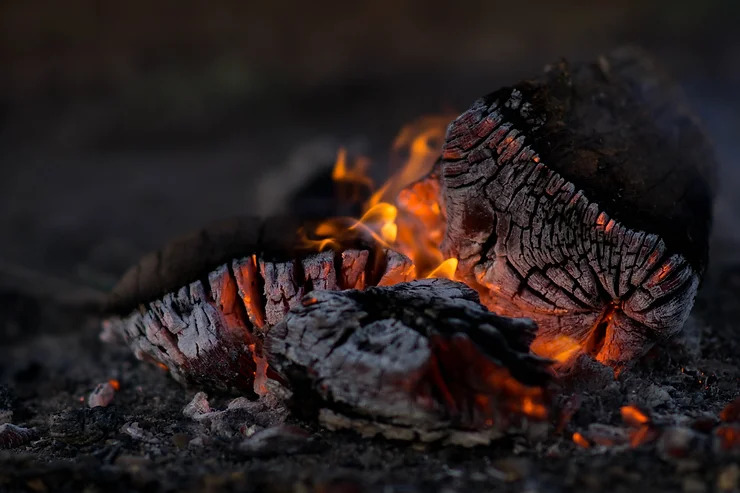
\includegraphics[scale=0.4]{Linn/ember2.jpg}
    \end{center}
    \caption{Hot ember cools by radiating heat to it's surroundings.}
    \label{fig:ember}
    \end{figure}
    
But in the case of stars, they are born in these places with cold gas called nebulae.\unsure{More correct might be to use molecular clouds?}
How can that happen? How can these huge furnaces that generate so much heat and light be born from these cold clouds of gas?

\subsection{Nuclear energy}
%Once we understand how much energy is produced by the Sun.
The Sun produces so much energy on a day to day basis that we are left wondering what could be the source of this energy.
Could it be something that caught fire a long time ago and is still burning?
Now we know that the answer is controlled thermonuclear fusion.
Nuclear energy was only known as a source of energy after the works of Einstein and others.
But even then we had to wait until the discovery of quantum mechanics and quantum tunnelling to emphatically say that this was the reason.\info{Confirmation of this theory comes from observations of neutrinos}
    \begin{figure}
    \begin{center}
	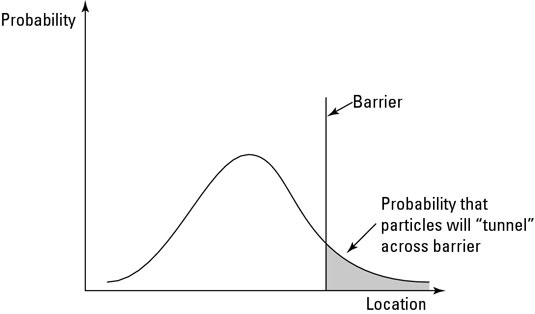
\includegraphics[scale=0.8]{Linn/tunnel.jpg}
    \end{center}
    \caption{Sketch showing quantum tunnelling.}
    \label{fig:}
    \end{figure}
    
\subsection{Plasma}
What do you expect the star to be made of ? Is it a solid orb made of metal? Is it gas or liquid? The answer is neither. The matter in stars exist in the fourth state of matter called plasma.
However the plasma can still be considered to behave like a perfect gas.
\info{Talk about presence of magnetic fields.}
However since plasma is composed of charged particles, the motion of plasma can create magnetic fields.
It is believed that the magnetic field in the stars are reponsible for the heating up of their atmospheres and for the transient events like flares and CMEs.
    \begin{figure}
    \begin{center}
	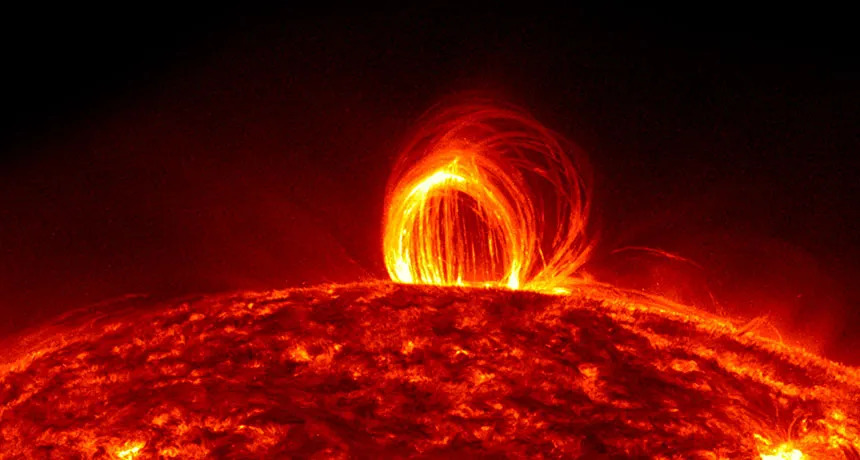
\includegraphics[scale=0.4]{Linn/coronal-rain_feat.jpg}
    \end{center}
    \caption{Blobs of plasma can fall like rain in the sun’s atmosphere, as seen in the center of this image of a solar flare from July 2012. Image Credit: NASA}
    \label{fig:plasma}
    \end{figure}



\begin{thebibliography}{4}
\providecommand{\natexlab}[1]{#1}
\providecommand{\url}[1]{\texttt{#1}}
\expandafter\ifx\csname urlstyle\endcsname\relax
  \providecommand{\doi}[1]{doi: #1}\else
  \providecommand{\doi}{doi: \begingroup \urlstyle{rm}\Url}\fi
\bibitem[1]{choudhuri_natures_2015}
Arnab~Rai Choudhuri.
\newblock \emph{Nature's Third Cycle: A Story of Sunspots}.
\newblock {Oxford University Press}, {Oxford ; New York}, 2015.
\newblock ISBN 978-0-19-967475-6.

\bibitem[2]{shu_physical_1982}
Frank~H. Shu.
\newblock \emph{The Physical Universe: An Introduction to Astronomy}.
\newblock A Series of Books in Astronomy. {Univ. Sience Books}, {Sausalito,
  Calif}, 9. print edition, 1982.
\newblock ISBN 978-0-935702-05-7.

\bibitem[3]{priest_magnetohydrodynamics_nodate}
Eric Priest.
\newblock Magnetohydrodynamics of {{The Sun}}.

\end{thebibliography}
\vspace{0.5cm}
\noindent\fbox{%
	\parbox{\textwidth}{%
		\textbf{About the Author}\vspace{0.2cm} \\
		\textbf{Linn Abraham} is a researcher in Physics, specializing in A.I. applications to astronomy. 
He is currently involved in the development of CNN based Computer Vision tools for
prediction of solar flares from images of the Sun, morphological classifications of galaxies from optical images surveys and radio galaxy source extraction from radio observations.
	}
}
    %</note>
    \printbibliography
\end{document}
